\documentclass[a4paper, 10pt]{article}
\usepackage[UTF8]{ctex}
\usepackage[vmargin=.75in,hmargin=.5in]{geometry}
\usepackage{multicol}
\usepackage{amsmath, amssymb, amsthm, bm, mathrsfs}
\allowdisplaybreaks[4] % 公式跨页 Cross-page equations
\providecommand{\abs}[1]{\left\lvert#1\right\rvert} % 绝对值 Absolute
\providecommand{\norm}[1]{\left\lVert#1\right\rVert} % 范数 Norm
\providecommand{\re}{\,\text{Re}\,} % 复数的实部 Real part of complex number
\providecommand{\im}{\,\text{Im}\,} % 复数的虚部 Imaginary part of complex number
\providecommand{\sgn}{\,\text{sgn}\,} % 符号函数 Sign function
\providecommand{\sinc}{\,\text{sinc}\,} % 辛格函数 sinc function
\providecommand{\bra}[1]{\left\langle#1\right\rvert} % 左矢 Bra
\providecommand{\ket}[1]{\left\lvert#1\right\rangle} % 右矢 Ket
\providecommand{\braket}[2]{\left\langle#1\left\vert\right.#2\right\rangle} % 右矢接左矢 Contiguous ket after bra
\providecommand{\tr}{\,\text{Tr}\,} % 右矢接左矢 Contiguous ket after bra
\usepackage{multirow}
\usepackage{graphicx}
\usepackage{float}
\usepackage{subfigure}
\begin{document}
\title{蔡氏电路中混沌现象的机制分析}
\author{陈稼霖\and 薛加民}
\date{2020 年 11 月 18 日}
\maketitle
\begin{abstract}
蔡氏电路是一种含有非线性元件的电路,在其演化的过程中,呈现出典型的混沌现象. 从分岔图、李雅普诺夫指数等角度均可验证蔡氏电路中的混沌现象,但这些方法仍停留在较为抽象的层面. 我们提出了一种对蔡氏电路演化机理的直观解释:将蔡氏电路视为一个自由度为$3$的系统,三个广义坐标确定了系统对应的相点在相空间中的位置,由基尔霍夫定律导出的描述蔡氏电路演化的微分方程组刻画了分布在相空间中的广义力场,相点受广义力作用在相空间中运动. 相空间中存在两个能够吸引相点的吸引子,它们相互竞争相点的归属权,从而使相点的演化呈现混沌现象. 吸引子对相点的吸引能力随蔡氏电路相关参数的改变而改变,这解释了相点演化轨迹的四种不同类型. 我们通过理论模拟与实验相结合的方法验证了上述观点,实验中还观察到了李萨如图跳变的现象,这进一步证实了吸引子对相点的竞争机制.
\end{abstract}

\begin{multicols*}{2}

\section{理论背景}
\subsection{混沌}
混沌(chaos)指的是无序、混乱的状态. 混沌的动力学系统,其演化虽然由确定的原理决定,在理论上可模拟,但由于微小的初始条件误差可导致演化路径的显著改变,从而导致无法准确地预测. 混沌非常普遍,其广泛地存在于力学系统(如三体问题、双杆摆、湍流)、生态系统(如虫口模型)、大气系统等各种体系中. 直至目前,对混沌并没有一个统一、公认的定义. 相对较为知名的,有 Robert L.~Devaney 提出的混沌动力学系统的三大性质\cite{hasselblatt2003first}:
\begin{itemize}
    \item[(1)] 对初始条件敏感;
    \item[(2)] 拓扑可传递;
    \item[(3)] 具有稠密的周期性轨道,
\end{itemize}
以及 James A.~Yorke 和他的学生李天岩提出的 Lee-Yorke 混沌定义\cite{tien1975period}:设$f(x)$是区间$[a,b]$上的连续自映射,其中$[a,b]$是$\mathbb{R}$的子区间,若满足以下三个条件,则为混沌:
\begin{itemize}
    \item[(1)] $f(x)$存在一切周期的周期点;
    \item[(2)] 存在一个不可数子集$S\subset[a,b]$,且$S$不含周期点,对任意$x_1,x_2\in S$,且$x_1\neq n_2$,有
    \begin{align}
        \lim_{n\rightarrow\infty}\inf\abs{f^n(x)-f^n(y)}=&0,\\
        \lim_{n\rightarrow\infty}\sup\abs{f^n(x)-f^n(y)}>&0;
    \end{align}
    \item[(3)] 对任意$x\in S$即$f$的任意周期点$p\in[a,b]$有
    \begin{align}
        \lim_{n\rightarrow\infty}\sup\abs{f^n(x)-f^n(p)}>0.
    \end{align}
\end{itemize}
尽管混沌没有公认的定义,但混沌系统往往具有一些普遍的特征,如:系统的演化方程(组)(时间连续系统的微分方程,或时间离散系统的差分方程)往往存在非线性项;分岔图表现出分形的特性;从分岔图中的分岔点间的相对位置关系可以得到费根鲍姆常数;存在周期为$3$的周期点;具有正的李雅普诺夫. 以这些特征为证据,我们可以大致判断出一个系统是否存在混沌.

\subsection{蔡氏电路}
蔡氏电路(Chua's Circuit)由蔡少棠与1983年发明,是一种包含非线性电阻的$LRC$电路,在适当的参数下,其演化过程呈现出典型的混沌现象. 图\ref{ChuaCircuit}(a)展示了一种蔡氏电路的实现方式,该电路通过一个电感$L$,两个电容$C_1,C_2$和一个非线性电阻$N_R$并联而成,此外还串联了一个可变电阻作为可变参数用于调整电路的状态. 电路中的非线性电阻(图\ref{ChuaCircuit}(b)),也称蔡氏二极管,是由两个负阻抗转换器并联得到,具有由分段函数表示的$I-V$曲线,是蔡氏电路非线性及其混沌现象的根本来源. 负阻抗转换器(图\ref{ChuaCircuit}(c))是个同时加上了正反馈和负反馈的运算放大器. 由于运放的输出电压受到供电电压的限制,因此负阻抗转换器的$I-V$关系(图\ref{ChuaCircuit}(e))表为分段函数:
\begin{align}
    I(V)=\left\{\begin{array}{ll}
        \frac{V-V_{\text{nn}}}{R_f},&V<\frac{R_b}{R_a+R_b}V_{nn},\\
        -\frac{R_a}{R_bR_f}V,&\frac{R_b}{R_a+R_b}V_{\text{nn}}\leq V\leq\frac{R_b}{R_a+R_b}V_{\text{pp}},\\
        \frac{V-V_{\text{pp}}}{R_f},&V>\frac{R_b}{R_a+R_b}V_{\text{pp}},
    \end{array}\right.
\end{align}
式中各变量对应物理量已在图\ref{ChuaCircuit}(c)中标出. 由两个负阻抗并联而成的蔡氏二极管的$I-V$关系(图\ref{ChuaCircuit}(d))即为两个负阻抗转换器各自对应$I-V$函数的加和:
\begin{align}
    I=f(V)=I_1(V)+I_2(V),
\end{align}
其中
\begin{align}
    I_1(V)=&\left\{\begin{array}{ll}
        \frac{V+V_2}{R_1},&V<-\frac{R_3}{R_2+R_3}V_1,\\
        -\frac{R_2}{R_3R_1}V,&-\frac{R_3}{R_2+R_3}V_1\leq V\leq\frac{R_3}{R_2+R_3}V_2,\\
        \frac{V-V_1}{R_1},&V>\frac{R_3}{R_2+R_3}V_2,\\
    \end{array}\right.\\
    I_2(V)=&\left\{\begin{array}{ll}
        \frac{V+V_5}{R_4},&V<-\frac{R_6}{R_5+R_6}V_1,\\
        -\frac{R_5}{R_6R_4},&-\frac{R_6}{R_5+R_6}V_1\leq V\leq\frac{R_6}{R_5+R_6}V_2,\\
        \frac{V-V_1}{R_4},&V>\frac{R_6}{R_5+R_6}V_2.
    \end{array}\right.
\end{align}

根据基尔霍夫定律,可以列出描述蔡氏电路演化的微分方程组:
\begin{align}
    \label{Kirchhoff-ode-1}
    \frac{\mathrm{d}V_{C1}}{\mathrm{d}t}=&-\frac{1}{C_1}\left[\frac{V_{C1}-V_{C2}}{R}+f(V_{C1})\right],\\
    \frac{\mathrm{d}V_{C2}}{\mathrm{d}t}=&-\frac{1}{C_2}\left[-\frac{V_{C1}-V_{C2}}{R}-I_L\right],\\
    \label{Kirchhoff-ode-3}
    \frac{\mathrm{d}I_L}{\mathrm{d}t}=&-\frac{1}{L}V_{C2},
\end{align}
其中$V_{C1}$和$V_{C2}$分别为电容$C_1$和$C_2$两端的电压,$I_L$为经过电容$L$的电流,微分方程组中的非线性项$f(V_{C1})$是混沌的根本来源.

\begin{figure}[H]
    \centering
    \includegraphics[width=\columnwidth]{ChuaCircuit.eps}
    \caption{蔡氏电路. (a) 蔡氏电路图;(b) 蔡氏二极管电路图;(c) 负阻抗转换器电路图;(d) 蔡氏二极管$I-V$曲线;(c) 负阻抗转换器$I-V$曲线.}
    \label{ChuaCircuit}
\end{figure}

\section{蔡氏电路混沌现象的验证}

\subsection{蔡氏电路演化路径的理论模拟}
根据上述微分方程组及蔡氏二极管的$I-V$关系,给定初始条件$V_{C1}(0)=0.01\mathrm{V}$,$V_{C2}(0)=-0.01\mathrm{V}$,$I_L(0)=0\mathrm{mA}$,改变可变电阻$R$的取值,模拟蔡氏电路的演化,共可得到四种类型的$(V_{C1},V_{C2})$点的轨迹:
\begin{itemize}
    \item[(1)] $0<R\leq 1543\,\Omega$ —— 单周期圆角平行四边形状轨迹:随着可变电阻阻值$R$的增大,圆角平行四边形的尺寸增大并且形状更加圆滑,如图\ref{Rounded-parallelogram};
    \begin{figure}[H]
        \centering
        \includegraphics[width=\columnwidth]{Rounded-parallelogram.eps}
        \caption{可变电阻$R$不同阻值时的圆角四边形状轨迹. 可变电阻阻值:(a) $R=10\,\Omega$;(b) $R=500\,\Omega$;(c) $R=1000\,\Omega$;(d) $R=1500\,\Omega$.}
        \label{Rounded-parallelogram}
    \end{figure}
    \item[(2)] $1544\,\Omega\leq R\leq 1934\,\Omega$ —— 双吸引子轨迹:$(V_{C1},V_{C2})$时而绕某一定点螺旋运动,时而绕另一点螺旋运动,在这两种螺旋运动模式间无明显规则地来回跳变,并且随着可变电阻阻值的增大,螺旋运动的轨道尺寸增大,轨道中央未被轨迹填充的空白区域从无到有,并不断扩大,如图\ref{Double-attractor};
    \begin{figure}[H]
        \includegraphics[width=\columnwidth]{Double-attractor.eps}
        \caption{可变电阻$R$不同阻值时的双吸引子轨迹. 可变电阻阻值:(a) $R=1600\,\Omega$;(b) $R=1700\,\Omega$;(c) $R=1800\,\Omega$;(d) $R=1900\,\Omega$.}
        \label{Double-attractor}
    \end{figure}
    \item[(3)] $1935\,\Omega\leq R\leq 2020\,\Omega$ —— 单吸引子轨迹:给定相同的初始条件下,$(V_{C1},V_{C2})$点绕某个顶点螺旋运动,随着可变电阻阻值$R$的增大,螺旋运动的轨道呈现出不同的交叠状况,大致趋势为周期数(轨道的层次数)由多周期变为单周期,而后又重新趋于多周期,在此过程中,偶尔会出现较小偶数周期数的情况,如图\ref{Single-attractor};
    \begin{figure}[H]
        \centering
        \includegraphics[width=\columnwidth]{Single-attractor.eps}
        \caption{可变电阻$R$不同阻值时的单吸引子轨迹. 可变电阻阻值和轨道周期数:(a) $R=1950\,\Omega$,多周期;(b) $R=1965\,\Omega$,多周期,但主要分为两簇;(c) $R=1967.5\,\Omega$,二周期;(d) $R=1970\,\Omega$,多周期,但主要分为两簇;(e) $R=1972\,\Omega$,多周期;(f) $R=1980\,\Omega$,单周期;(g) $R=1990\,\Omega$,多周期,但主要分为两簇;(h) $R=1994\,\Omega$,四周期;(i) $R=1998\,\Omega$,二周期;(j) $R=2004\,\Omega$,多周期;(k) $R=2006\,\Omega$,二周期;(l) $R=2008\,\Omega$,多周期.}
        \label{Single-attractor}
    \end{figure}
    \item[(4)] $R\geq 2021\,\Omega$ —— 轨迹收敛至一点:如图\ref{Converge}.
    \begin{figure}[H]
        \centering
        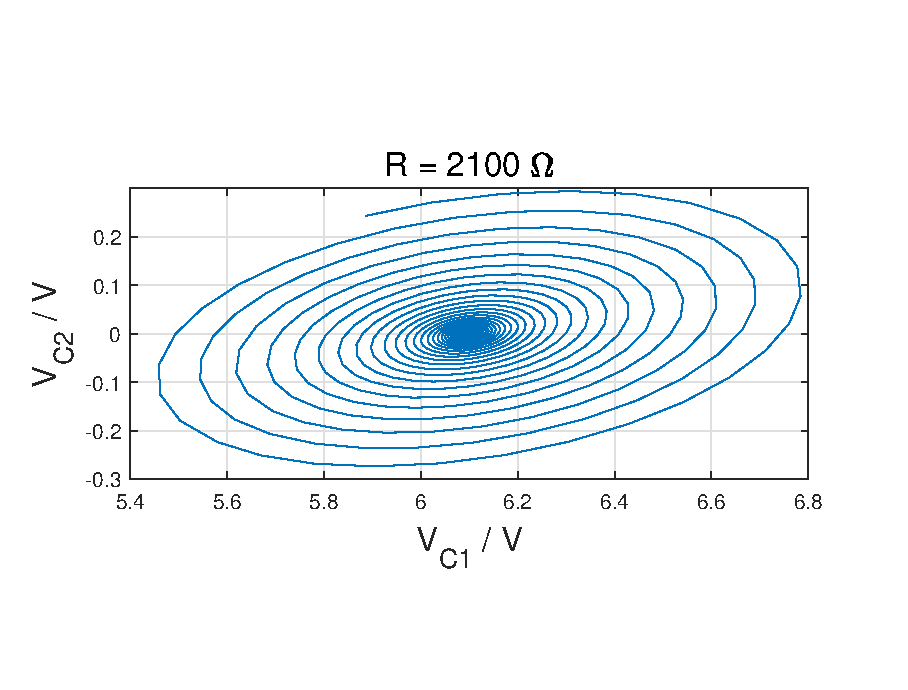
\includegraphics[width=.8\columnwidth]{R=2100.eps}
        \caption{可变电阻阻值$R=2100\,\Omega$时,蔡氏电路的$(V_{C1},V_{C2})$点轨迹收敛至一点.}
        \label{Converge}
    \end{figure}
\end{itemize}

蔡氏电路的演化轨迹对初始条件极为敏感,这在单吸引子阶段体现得尤为显著. 如图\ref{InitialConditionSensitivity}所示,蔡氏电路在设定可变电阻$R=1950\Omega$,$V_{C1}(0)=0.01\mathrm{V}$,$V_{C2}(0)=-0.01\mathrm{V}$,$I_L(0)=0\mathrm{mA}$和$V_{C1}(0)=-0.01\mathrm{V}$,$V_{C2}(0)=0.01\mathrm{V}$,$I_L(0)=0\mathrm{mA}$两种初始条件下的$(V_{C1},V_{C2})$点呈现出两种截然不同的轨迹:前者主要在$V_{C1}-V_{C2}$的左半平面做螺旋运动,而后者主要在$V_{C1}-V_{C2}$的右半平面做螺旋运动.

\begin{figure}[H]
    \centering
    \subfigure[初始条件:$V_{C1}(0)=0.01\mathrm{V}$,$V_{C2}(0)=-0.01\mathrm{V}$,$I_L(0)=0\mathrm{mA}$.]{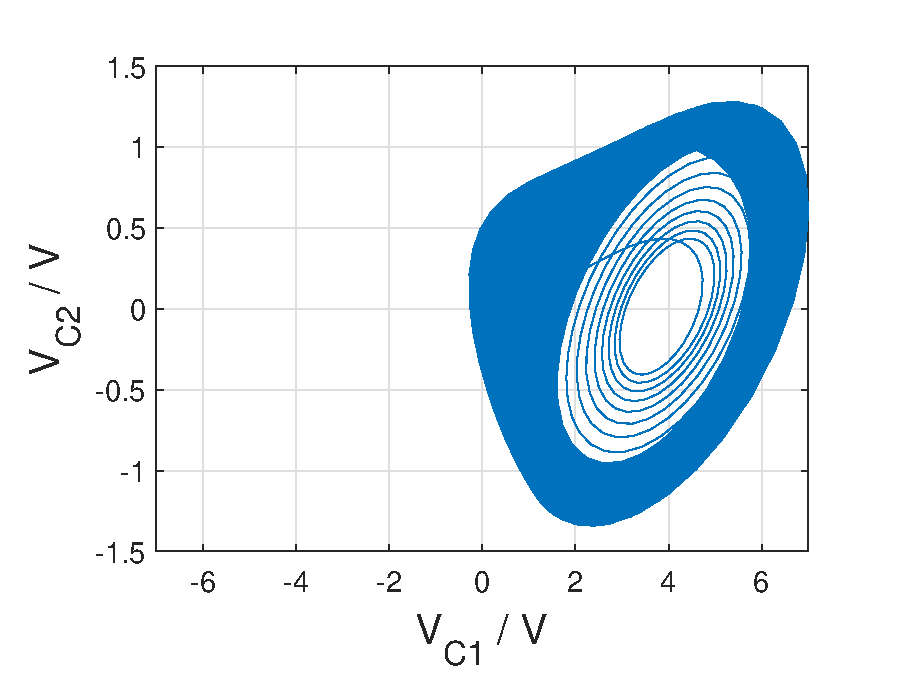
\includegraphics[width=.48\columnwidth]{R=1950,y0=[0.01,-0.01,0].eps}}
    \subfigure[初始条件:$V_{C1}(0)=-0.01\mathrm{V}$,$V_{C2}(0)=0.01\mathrm{V}$,$I_L(0)=0\mathrm{mA}$.]{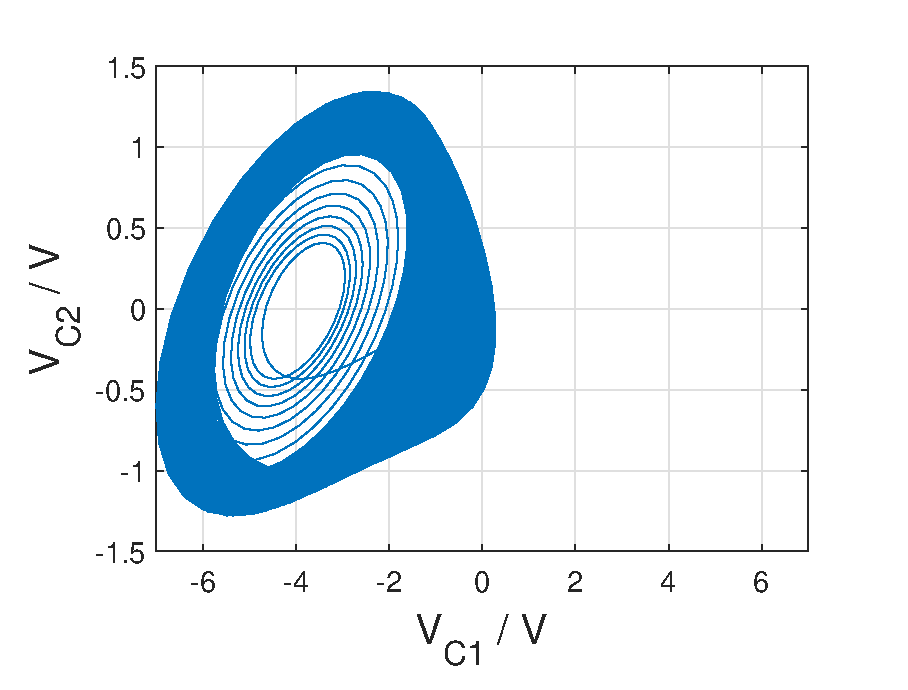
\includegraphics[width=.48\columnwidth]{R=1950,y0=[-0.01,0.01,0].eps}}
    \caption{可变电阻$R=1950\,\Omega$时,蔡氏电路在不同初始条件下$(V_{C1},V_{C2})$点轨迹.}
    \label{InitialConditionSensitivity}
\end{figure}

\subsection{分岔图中的费根鲍姆常数和三周期}
对于非线性系统在不同参数下的演化,我们总是可以以变化系统参数为横坐标,以表示系统状态的某个因变量为纵坐标,绘制出分岔图. 1975年,费根鲍姆发现分岔图中相邻分岔点间隔的比值总是趋于某无理常数,其中相邻分岔点水平方向上距离之比称为第一费根鲍姆常数,其值为$\delta=4.6692016091\cdots$,竖直方向上距离之比称为第二费根鲍姆常数,其值为$\alpha=2.502907875\cdots$.

为了验证蔡氏电路的分岔图的相邻分岔点距离之比同样趋于费根鲍姆常数,我们以可变电阻阻值$R$作为系统参数,以$V_{C1}$在演化过程中的极大值作为系统状态,模拟出可变电阻阻值$R\in[1920\,\Omega,2020\,\Omega]$的分岔图,如图\ref{Bifurcation}(a)所示. 在$R\in[1934\,\Omega,2020\,\Omega]$的范围内,可以看出蔡氏电路的周期数随着可变电阻阻值$R$的增大,先从多周期减为单周期,而后又有单周期增至多周期的大致趋势,期间可以隐约看出局部范围内周期数有分岔或成簇的情况. 但或许是由于微分方程求解方法精度不足,分岔图中的分岔不够清晰,故无法计算费根鲍姆常数. 在$R\in[1960\,\Omega,2000\,\Omega]$范围内进行更精细的模拟,得到如图\ref{Bifurcation}(b)所示的分岔图. 该分岔图仍然未能达到可计算费根鲍姆常数的程度,但可以观察到,单周期区间($[1975\,\Omega,1987\,\Omega]$)之前,在$R=1967\,\Omega$附近存在明显的双周期,单周期区间之后,在$R=1994\,\Omega$附近出现了明显的四周期,在$R=1998\,\Omega$附近出现了明显的双周期. 最重要的是,在$R=1992\,\Omega$附近出现了三周期. 已被证明\cite{tien1975period},三周期轨道的出现意味着混沌的存在,因此从这一角度可以佐证,蔡氏电路这一系统是混沌的. 若模拟并绘制$R=1992\,\Omega$附近的蔡氏电路的$(V_{C1},V_{C2})$点轨迹,可以发现仍然可能在局部存在四条轨迹,但其中某两条轨迹高度重合,这可能是求解微分方程组的精度不足所导致的.

\begin{figure}[H]
    \centering
    \includegraphics[width=\columnwidth]{Bifurcation.eps}
    \caption{蔡氏电路的分岔图,以可变电阻阻值$R$为系统参数,以$V_{C1}$在演化过程中的极大值为系统状态. (a) 可变电阻阻值范围$R\in[1920\,\Omega,2020\,\Omega]$;(b) 可变电阻阻值范围$R\in[1960\,\Omega,2000\,\Omega]$.}
    \label{Bifurcation}
\end{figure}

\subsection{李雅普诺夫指数}
李雅普诺夫指数$\lambda$刻画了初始条件的微小差异导致的演化轨迹的差异程度. 在给定初始条件的微小差异$\delta y(0)$下,经过时间间隔$t$的演化后,系统状态的差距$\abs{\delta y(t)}$表为
\begin{align}
    \abs{\delta y(t)}=e^{\lambda t}\abs{\delta y(0)}.
\end{align}
通常,我们感兴趣的是最大李雅普诺夫指数:
\begin{align}
    \lambda=\lim_{t\rightarrow\infty}\lim_{\delta y(0)\Rightarrow 0}\frac{1}{t}\ln\frac{\abs{\delta y(t)}}{\abs{\delta y(0)}}.
\end{align}
最大李雅普诺夫指数是表征混沌存在与否的一个重要特征量. 最大李雅普诺夫指数$\lambda>0$,则表明初始条件的微小差异会导致一段时间后演化轨迹的截然不同,即系统对初始条件敏感,处于混沌的状态,且$\lambda$越大表明,系统对初始条件越敏感;反之,初始条件的差异并不会随着系统的演化而扩大,即使在初始条件有一定误差的情况下系统仍可以被较好地预测,故不存在混沌.

利用 Wolf 法\cite{wolf1985determining},我们首先给定初始条件$V_{C1}=0.01\,\mathrm{V}$,$V_{C2}=-0.01\,\mathrm{V}$,$I_L=0\,\mathrm{mA}$,计算了可变电阻阻值在$R\in[1960\,\Omega,2000\,\Omega]$的不同取值下,蔡氏电路$V_{C1},V_{C2}$和$I_L$的最大李雅普诺夫指数,如图\ref{LyapunovExponent-R}(a). 从中可见,$V_{C1}$的最大李雅普诺夫指数除了$R$接近$2200\,\Omega$的范围外均保持正值,$V_{C2}$的最大李雅普诺夫指数除了$R\in[1544\,\Omega,1934\,\Omega]$范围内的局部区域以外均为负,$I_L$的最大李雅普诺夫指数整个计算范围内均为负,这说明除了$(V_{C1},V_{C2})$点轨迹收敛至一点的情况外,蔡氏电路均处于混沌状态,其中对初始条件敏感的主要是$V_{C1}$,而非$V_{C2}$和$I_L$,这与我们在第2.1小节中模的模拟结果相吻合,$(V_{C1},V_{C2})$点的轨迹覆盖的$V_{C1}$取值范围显著大于$V_{C2}$. 在$R\in[1544\,\Omega,1934\,\Omega]$范围内,$V_{C1},V_{C2}$和$I_L$的最大李雅普诺夫指数均显著高于其他范围内的最大李雅普诺夫指数,这说明双吸引子轨迹的演化对初始条件最为敏感. 对$R\in[1960\,\Omega,2000\,\Omega]$范围内(对应$(V_{C1},V_{C2})$点轨迹为单吸引子)的最大李雅普诺夫指数进行更精细的计算,在轨迹周期数较小的$R$处$V_{C1}$的最大李雅普诺夫指数达到较大的值,如在$R=1967\,\Omega$附近,$(V_{C1},V_{C2})$点轨迹为二周期,对应$V_{C1}$的最大李雅普诺夫指数达到一尖锐的最大值,在$R\in[1975\,\Omega,1987\,\Omega]$范围内,$(V_{C1},V_{C2})$点轨迹保持单周期,对应$V_{C1}$的最大李雅普诺夫指数保持在较高的水平,这说明轨迹周期数越小,蔡氏电路的演化对初始条件越敏感. 我们还尝试选用初始条件$V_{C1}=0\,\mathrm{V}$,$V_{C2}=0\,\mathrm{V}$,$I_L=0\,\mathrm{mA}$,做了相同的计算,如图\ref{LyapunovExponent-R}(c)(d). 相对于初始条件$V_{C1}(0)=0.01\,\mathrm{V}$,$V_{C2}(0)=-0.01\,\mathrm{V}$,$I_L=0\,\mathrm{mA}$,初始条件$V_{C1}(0)=0\,\mathrm{V}$,$V_{C2}=0\,\mathrm{V}$,$I_L=0\,\mathrm{V}$下,$V_{C1}$的最大李雅普诺夫指数更大,变化也更平滑,并且即使在$R\geq 2021\,\Omega$范围仍然为正,说明蔡氏电路的演化对初始条件更敏感.

\begin{figure}[H]
    \centering
    \includegraphics[width=\columnwidth]{LyapunovExponent-R.eps}
    \caption{蔡氏电路的$V_{C1},V_{C2}$和$I_L$的最大李雅普诺夫指数随可变电阻阻值$R$的变化关系,垂直虚线代表不同类型$(V_{C1},V_{C2})$点轨迹转换的临界$R$值. (a) $R\in[500,2200]$,初始条件$V_{C1}(0)=0.01\,\mathrm{V}$,$V_{C2}(0)=-0.01\,\mathrm{V}$,$I_L=0\,\mathrm{A}$;(b) $R\in[1960\,\Omega,2000\,\Omega]$,初始条件$V_{C1}(0)=0.01\,\mathrm{V}$,$V_{C2}(0)=0.01\,\mathrm{V}$,$I_L=0\,\mathrm{mA}$;(c) $R\in[500\,\Omega,2200\,\Omega]$,初始条件$V_{C1}(0)=0\,\mathrm{V}$,$V_{C2}(0)=0\,\mathrm{V}$,$I_L=0\,\mathrm{mA}$;(d) $R\in[1960\,\Omega,2200\,\Omega]$,初始条件$V_{C1}(0)=0\,\mathrm{V}$,$V_{C2}(0)=0\,\mathrm{V}$,$I_L(0)=0\,\mathrm{mA}$.}
    \label{LyapunovExponent-R}
\end{figure}

上面的比较说明,不仅不同系统参数可以导致不同的最大李雅普诺夫指数,不同的初始条件对应的最大李雅普诺夫指数也是不同的. 为了验证这一点,我们给定可变电阻的阻值$R=1950\,\Omega$和初始时刻通过电感$L$的电流$I_L(0)=0$,计算从不同$V_{C1}(0)$和$V_{C2}(0)$出发开始演化的蔡氏电路的$V_{C1}$的最大李雅普诺夫指数,如图\ref{LyapunovExponentMap}所示. 我们发现无论初始条件如何,$V_{C1}$的最大李雅普诺夫指数,$V_{C1}$的李雅普诺夫指数始终为正数,其中初始条件为$V_{C1}(0)=0$,$V_{C2}(0)=0$,$I_L(0)=0$时对应的$V_{C1}$的最大李雅普诺夫显著大于其他初始条件对应的$V_{C1}$的最大李雅普诺夫指数.

\begin{figure}[H]
    \centering
    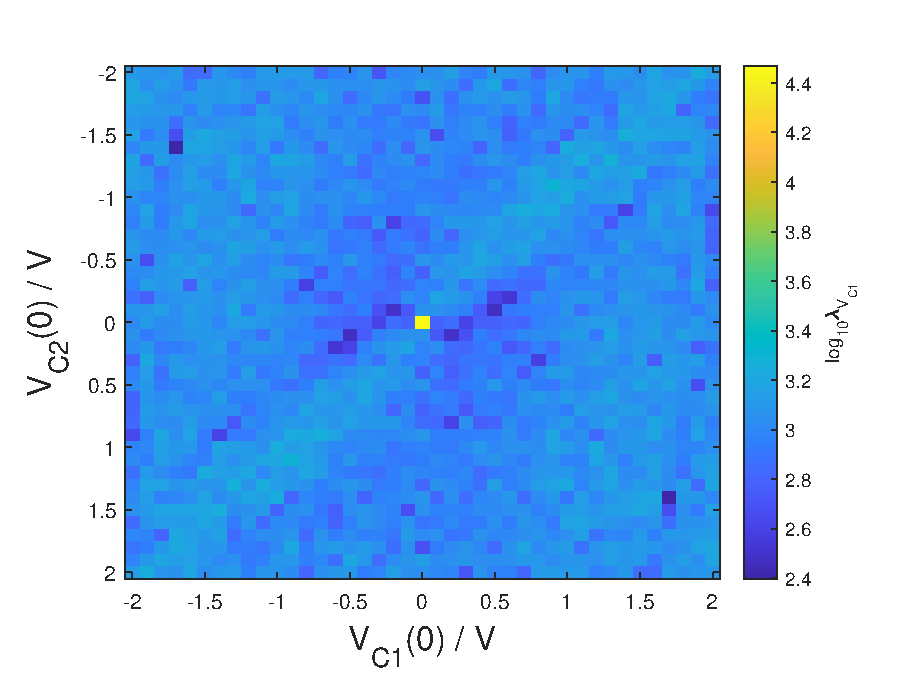
\includegraphics[width=\columnwidth]{LyapunovExponentMap.eps}
    \caption{不同初始条件$V_{C1}(0)$和$V_{C2}(0)$对应的蔡氏电路的$V_{C1}$的最大李雅普诺夫指数的常用对数.}
    \label{LyapunovExponentMap}
\end{figure}

\section{蔡氏电路演化机制的直观解释}

虽然我们从分岔图的三周期以及李雅普诺夫指数都验证了蔡氏电路混沌现象的存在,但是这些方法仍停留在较为抽象的层面,对形象理解蔡氏电路的演化机制及其混沌现象的出现帮助有限. 在此,我们提出了一种对于蔡氏电路演化机理的直观解释:蔡氏电路是一个自由度为$3$的动力学系统,该系统的一组广义坐标$V_{C1},V_{C2}$和$I_L$确定了系统状态所对应的相点在相空间中的位置,这三个变量的变化遵循常微分方程组\eqref{Kirchhoff-ode-1}-\eqref{Kirchhoff-ode-3},化为线性代数形式即
\begin{align}
    \frac{\mathrm{d}}{\mathrm{d}t}\left[\begin{matrix}
        V_{C1}\\
        V_{C2}\\
        I_L
    \end{matrix}\right]=A\left[\begin{matrix}
        V_{C1}\\
        V_{C2}\\
        I_L
    \end{matrix}\right]+b(V_{C1})
\end{align}
其中
\begin{align}
    A=\left[\begin{matrix}
        -\frac{1}{C_1R}&\frac{1}{C_2R}&0\\
        \frac{1}{C_2R}&-\frac{1}{C_2R}&\frac{1}{C_2}\\
        0&-\frac{1}{L}&0
    \end{matrix}\right]
\end{align}
和
\begin{align}
    b=\left[\begin{matrix}
        f(V_{C1})\\
        0\\
        0
    \end{matrix}\right]
\end{align}
刻画了分布在相空间中的广义力场,相点$[\begin{smallmatrix}
    V_{C1}&V_{C2}&I_L
\end{smallmatrix}]$受广义力场(产生的加速度)为
\begin{align}
    \frac{\mathrm{d}^2}{\mathrm{d}t^2}\left[\begin{matrix}
        V_{C1}\\
        V_{C2}\\
        I_L
    \end{matrix}\right]=A^2\left[\begin{matrix}
        V_{C1}\\
        V_{C2}\\
        I_L
    \end{matrix}\right]+Ab+\frac{\mathrm{d}b}{\mathrm{d}V_{C1}}\frac{\mathrm{d}V_{C1}}{\mathrm{d}t}.
\end{align}
上式右边最后一项幅值较小,在以下的模拟中忽略,而仅考虑前两项.

在相空间的某些点上,相点受广义力为零,其坐标满足
\begin{align}
    \frac{\mathrm{d}^2}{\mathrm{d}t^2}\left[\begin{matrix}
        V_{C1}\\
        V_{C2}\\
        I_L
    \end{matrix}\right]=0\Longrightarrow A\left[\begin{matrix}
        V_{C1}\\
        V_{C2}\\
        I_L
    \end{matrix}\right]+b=0.
\end{align}
这些点是相空间中的平衡点,数学上即对应微分方程组的不动点. 由于$b$是关于$V_{C1}$的、在$\left(-\infty,\min\left\{-\frac{R_3}{R_3+R_2}V_1,\frac{R_6}{R_6+R_5}V_1\right\}\right)$,$\left[\min\left\{-\frac{R_3}{R_3+R_2}V_1,\frac{R_6}{R_6+R_5}V_1\right\},\max\left\{-\frac{R_3}{R_3+R_2}V_1,-\frac{R_6}{R_6+R_5}V_1\right\}\right)$,$\left[\max\left\{-\frac{R_3}{R_3+R_2}V_1,-\frac{R_6}{R_6+R_5}V_1\right\},\min\left\{\frac{R_3}{R_3+R_2}V_2,\frac{R_6}{R_6+R_5}V_2\right\}\right]$,$\left(\min\left\{\frac{R_3}{R_3+R_2}V_2,\frac{R_6}{R_6+R_5}V_2\right\},\max\left\{\frac{R_3}{R_2+R_3}V_2,\frac{R_6}{R_6+R_5}V_2\right\}\right]$,$\left(\min\left\{\frac{R_3}{R_3+R_2}V_2,\frac{R_6}{R_6+R_5}V_2\right\},+\infty\right)$这五个区间(下称区间$\mathcal{R}_{-2}$,$\mathcal{R}_{-1}$,$\mathcal{R}_0$,$\mathcal{R}_1$,$\mathcal{R}_2$)上分别定义的分段函数,因此相空间中共有$5$个满足上式的平衡点. 这些平衡点的平衡类型直接决定相点在不动点周围的运动模式,值得我们关注. 若平衡点周围的广义力均有指向不动点的分量,则该平衡点处为稳定平衡,就有概率束缚住附近的相点,使其围绕在平衡点周围演化,这就形成了所谓的吸引子;若平衡点周围某处存在广义力有背离不动点的分量,则该平衡点处为不稳定平衡,处于该平衡点上的相位难以停留在不动点附近,也就无法形成吸引子. 当然,若平衡点当地和附近的广义力场较小,则相点会有较大概率演化至距平衡点较远处,此时距平衡点较远处的广义力场分布情况也将对相点的演化轨迹有较显著的影响.

我们对照模拟得到的蔡氏电路的$(V_{C1},V_{C2})$轨迹及轨迹上各点所受广义力在$V_{C1}-V_{C2}$平面上的投影,可以解释四种轨迹形成的机制:
\begin{itemize}
    \item[(1)] $0<R\leq 1543\,\Omega$ —— 单周期圆角平行四边形:如图\ref{Generalized-force-R=1500},中间三个个平衡点较为靠近,相点轨迹上广义力在$V_{C1}-V_{C2}$上的投影在区间$\mathcal{R}_1$,$\mathcal{R}_2$,$\mathcal{R}_3$虽然指向平衡点,但强度较小,故相点不局限在在平衡点附近做小范围运动,其运动轨迹可以涉及从$\mathcal{R}_{-2}$至$\mathcal{R}_2$的全部五个区间. $\mathcal{R}_{-2}$和$\mathcal{R}_2$这两个外围区间上有较大的回复力,可以将相点拉回中间的三个区间. 相点轨迹上广义力在$I_L-V_{C2}$平面上的投影较为均匀,且持续指向中间的平衡点,这或许可以解释轨迹的单周期的特征. 可变电阻在电路中起到了能量耗散的作用,它阻碍$V_{C1},V_{C2}$和$I_L$快速变化,换言之,可变电阻阻值的增大削弱了相点在相空间中的运动能力,而使平衡点对相点的吸引作用相应地增强,从而使得圆角平行四边形尺寸变小.
    \begin{figure}[H]
        \centering
        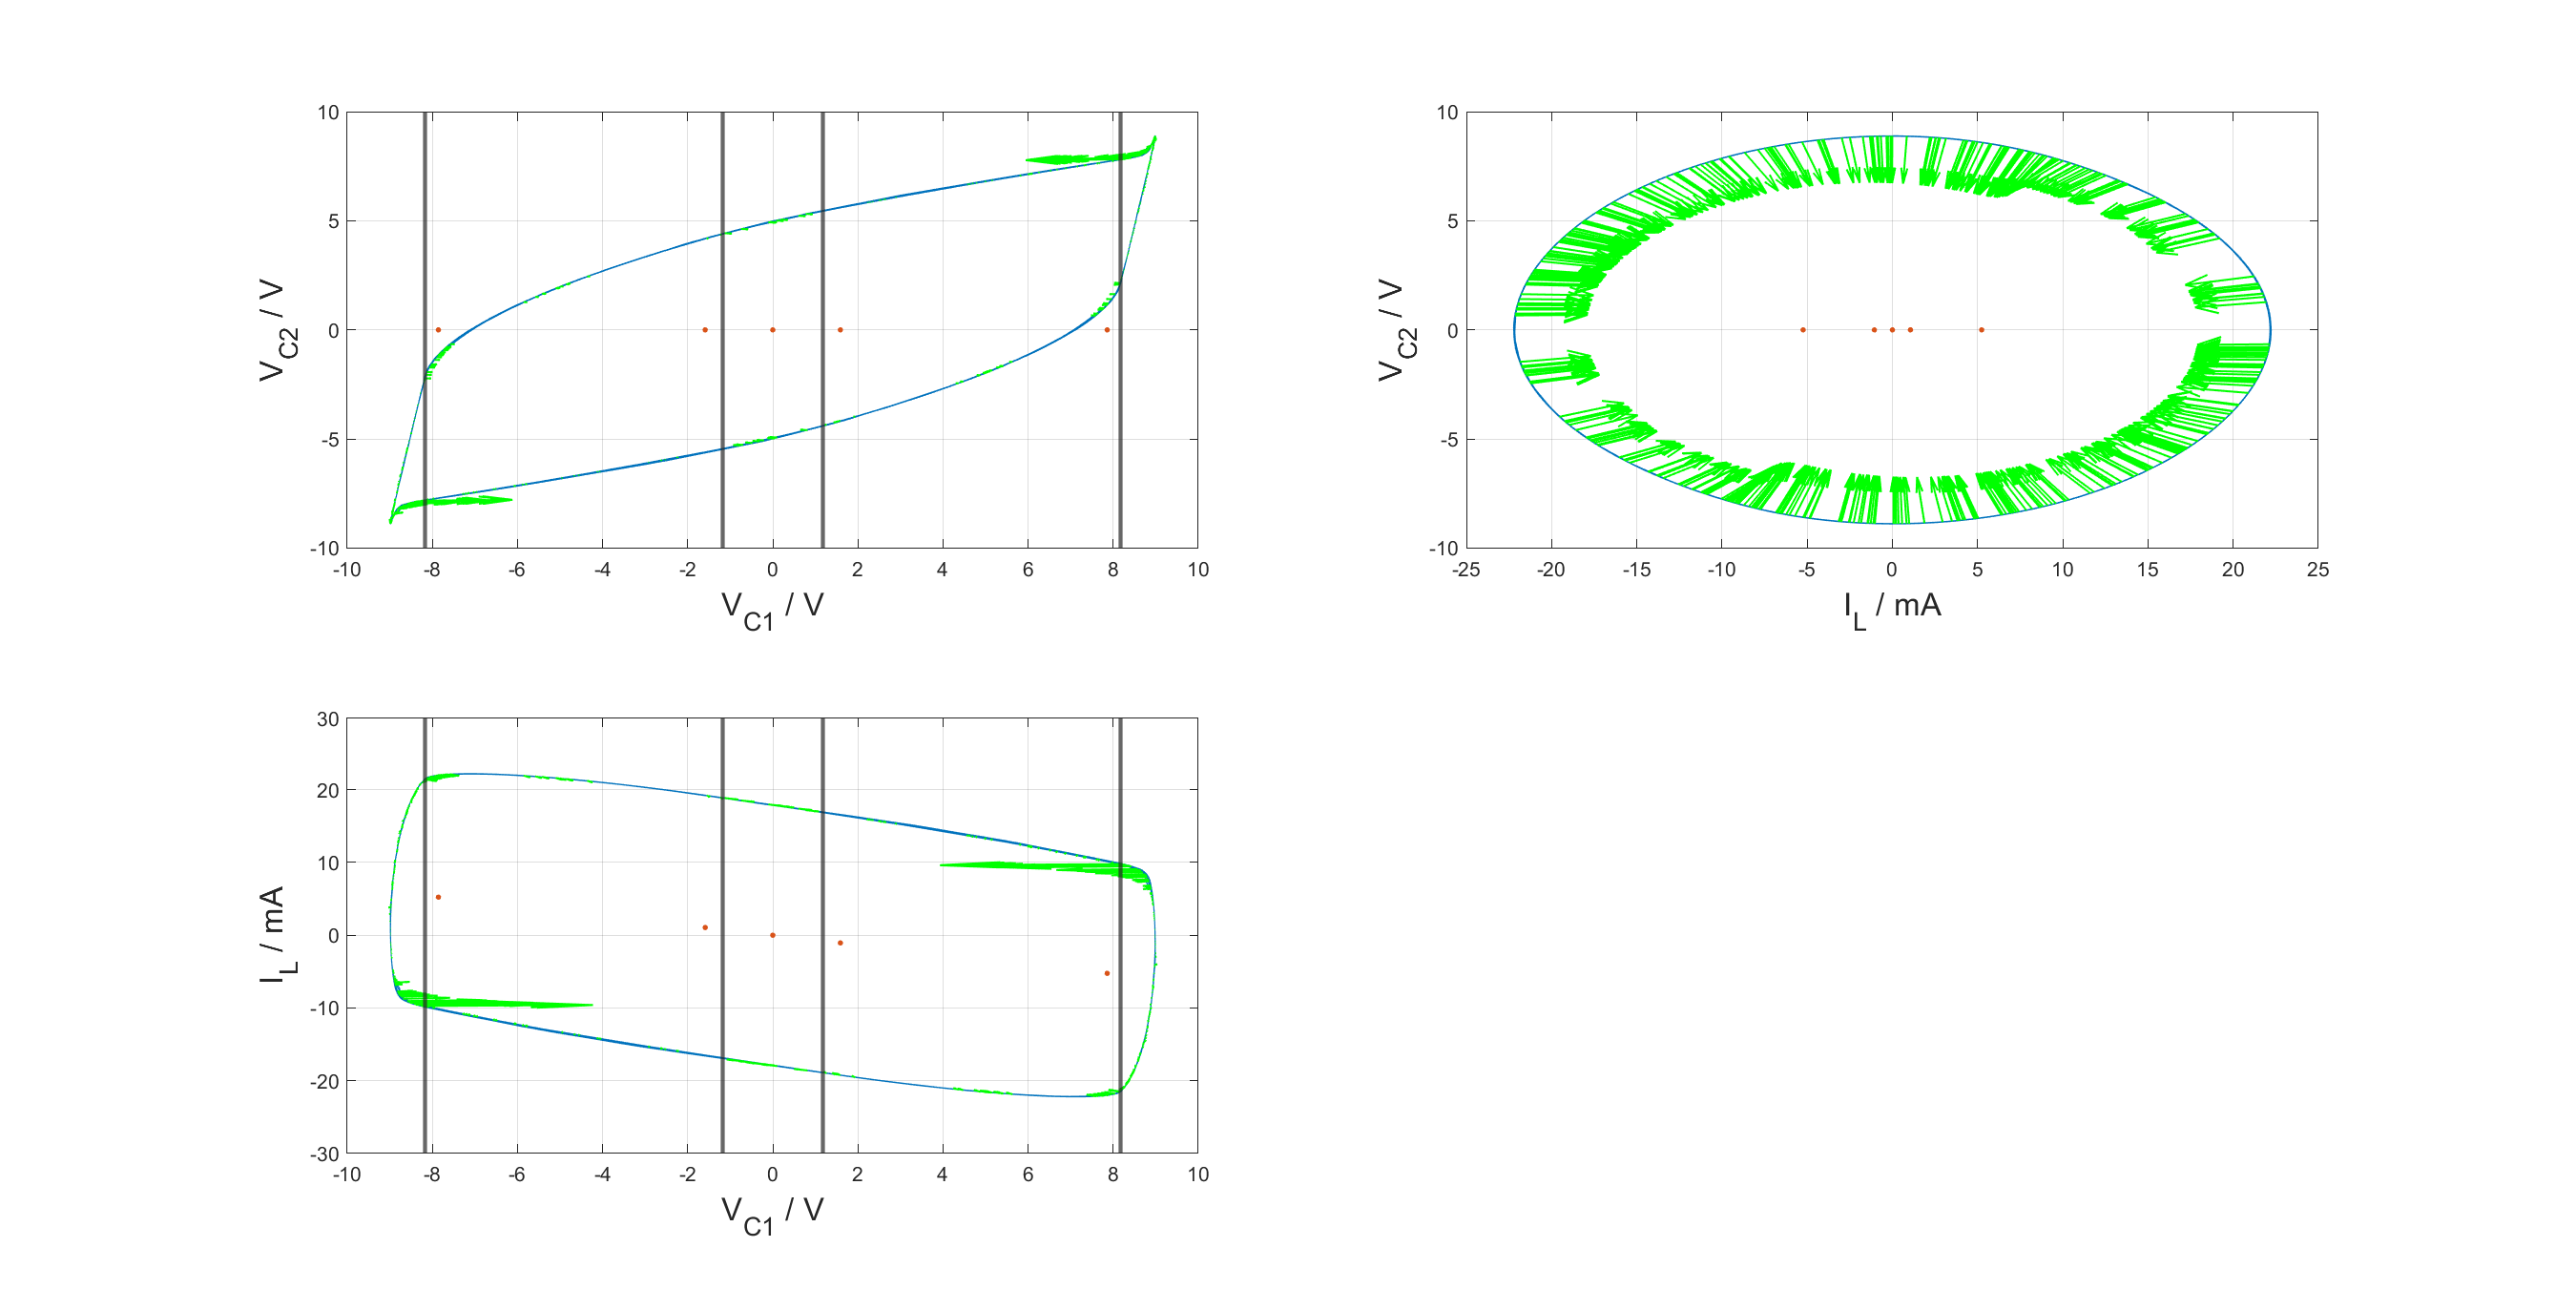
\includegraphics[width=\columnwidth]{Generalized-force-R=1500.eps}
        \caption{可变电阻阻值$R=1500\,\Omega$时,相点演化轨迹(蓝色实线)的三视图、五个平衡点(红点)及相点在轨迹各处受到的广义力在对应平面上的投影(绿色箭头).}
        \label{Generalized-force-R=1500}
    \end{figure}
    \item[(2)] $1544\,\Omega\leq R\leq 1934\,\Omega$ —— 双吸引子轨迹:如图\ref{Generalized-force-R=1800},$\mathcal{R}_{-1}$和$\mathcal{R}_1$区间的两个平衡点附近相点轨道上的广义力均指向对应的平衡点,而$\mathcal{R}_0$区间的平衡点(恰好为原点)附近相点轨道上的广义力则没有明显指向平衡点的规律,因此$\mathcal{R}_{-1}$和$\mathcal{R}_1$两个区间的平衡点具有一定束缚相点的能力. 而这一阶段的可变电阻阻值相对上一阶段有所增加,两个平衡点有足够的吸引能力使得相点在一段时间内绕其演化,从而形成吸引子,而$\mathcal{R}_0$区间上的平衡点则无法有效吸引相点形成吸引子. 此时,平衡点对相点的吸引力还相对较弱,因此相点在绕某一吸引子演化时有一定几率进入另一吸引子主导的区域而开始绕另一吸引子演化,这就形成了双吸引子的相点演化轨迹.
    \begin{figure}[H]
        \centering
        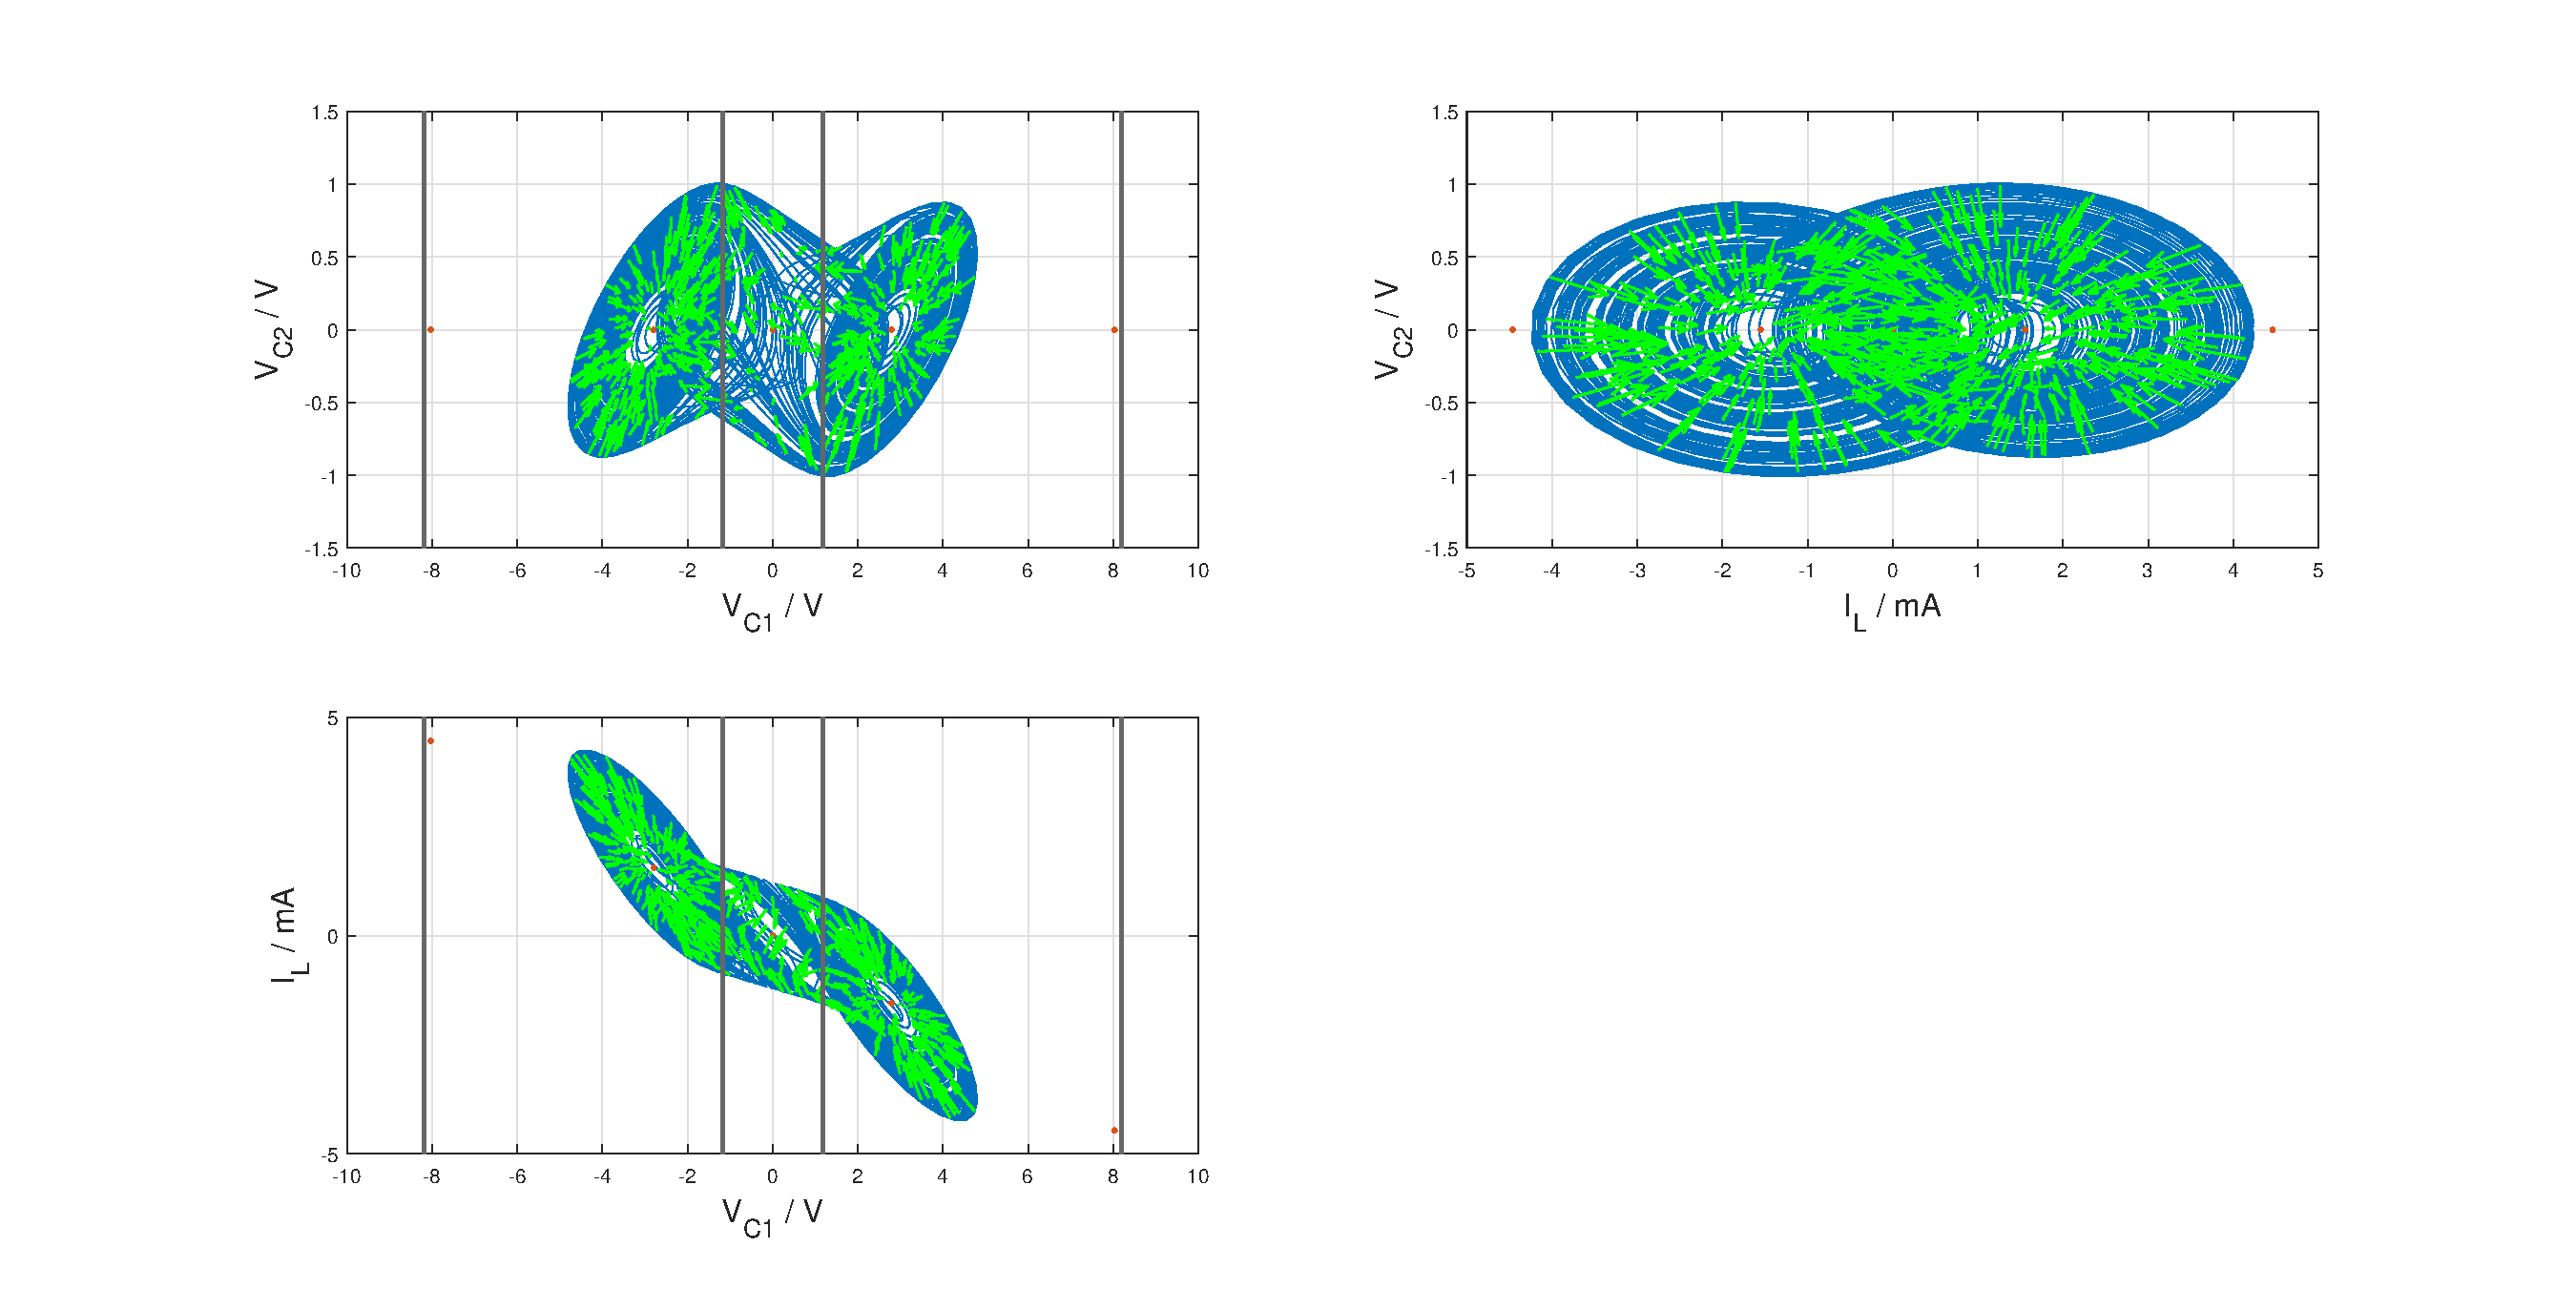
\includegraphics[width=\columnwidth]{Generalized-force-R=1800.eps}
        \caption{可变电阻阻值$R=1800\,\Omega$时,相点演化轨迹(蓝色实线)的三视图、五个平衡点(红点)及相点在轨迹各处受到的广义力在对应平面上的投影(绿色箭头).}
        \label{Generalized-force-R=1800}
    \end{figure}
    \item[(3)] $1935\,\Omega\leq R\leq 2020\,\Omega$ —— 单吸引子轨迹:如图\ref{Generalized-force-R=1950},这一阶段的可变电阻阻值进一步增加,平衡点的吸引能力相对于相点的运动能力进一步增强,此时相点一旦被某一平衡点所俘获就几乎没有逃出其控制的概率,从而形成单吸引子轨迹. 蔡氏电路演化的初始条件决定了相点最先倾向与哪一个平衡点,也就决定了相点此后围绕哪一个平衡点演化. 因此,初始条件的微小变动可能带来演化轨迹的截然不同,这解释了图\ref{InitialConditionSensitivity}展示的相点演化轨迹对初始条件的敏感性;两个平衡点对相点的吸引作用在原点达到平衡,因此从原点附近开始演化的相点轨迹对初始条件微小变动的敏感程度高于从其他初始条件开始演化的情况,这解释了图\ref{LyapunovExponentMap}中原点处$V_{C1}$的最大李雅普诺夫指数显著高于其他区域的情况.
    \begin{figure}[H]
        \centering
        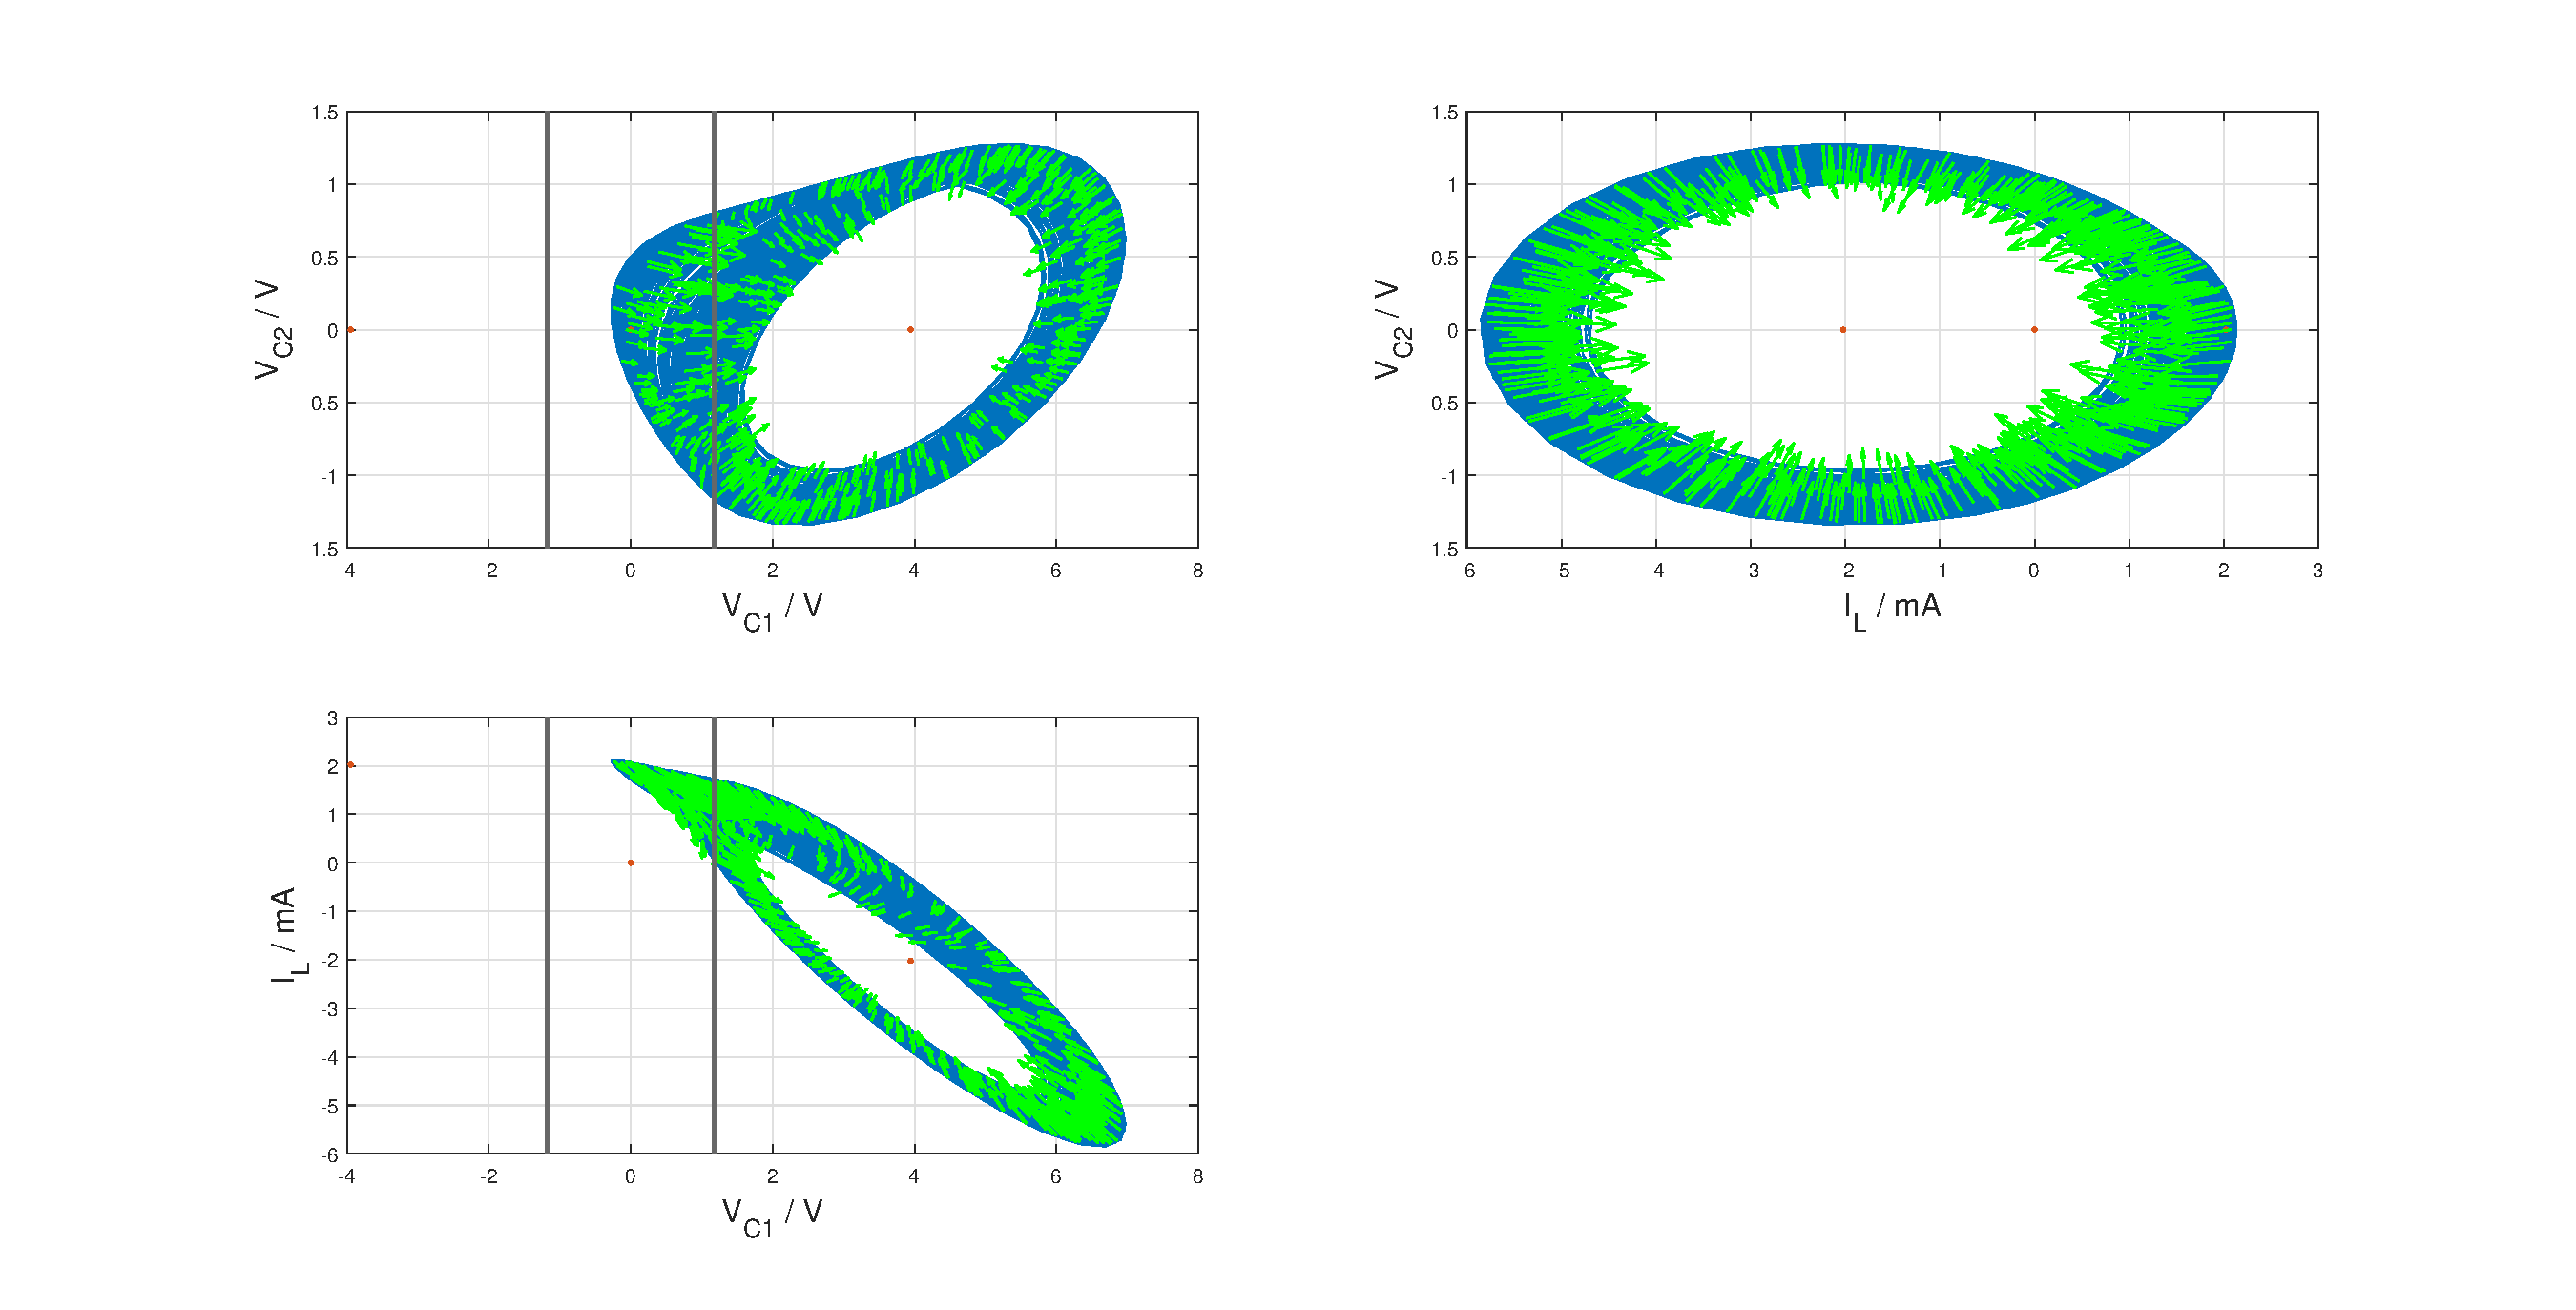
\includegraphics[width=\columnwidth]{Generalized-force-R=1950.eps}
        \caption{可变电阻阻值$R=1950\,\Omega$时,相点演化轨迹(蓝色实线)的三视图、平衡点(红点)及相点在轨迹各处受到的广义力在对应平面上的投影(绿色箭头).}
        \label{Generalized-force-R=1950}
    \end{figure}
    \item[(4)] $R\geq 2021\,\Omega$ —— 轨迹收敛至一点:这一阶段可变电阻的阻值进一步增大,因而平衡点的吸引力对相点的作用效果更为显著. 相点不再有围绕平衡点演化的动力,而是最终无限接近于平衡点,形成收敛于某一平衡点的轨迹.
    \begin{figure}[H]
        \centering
        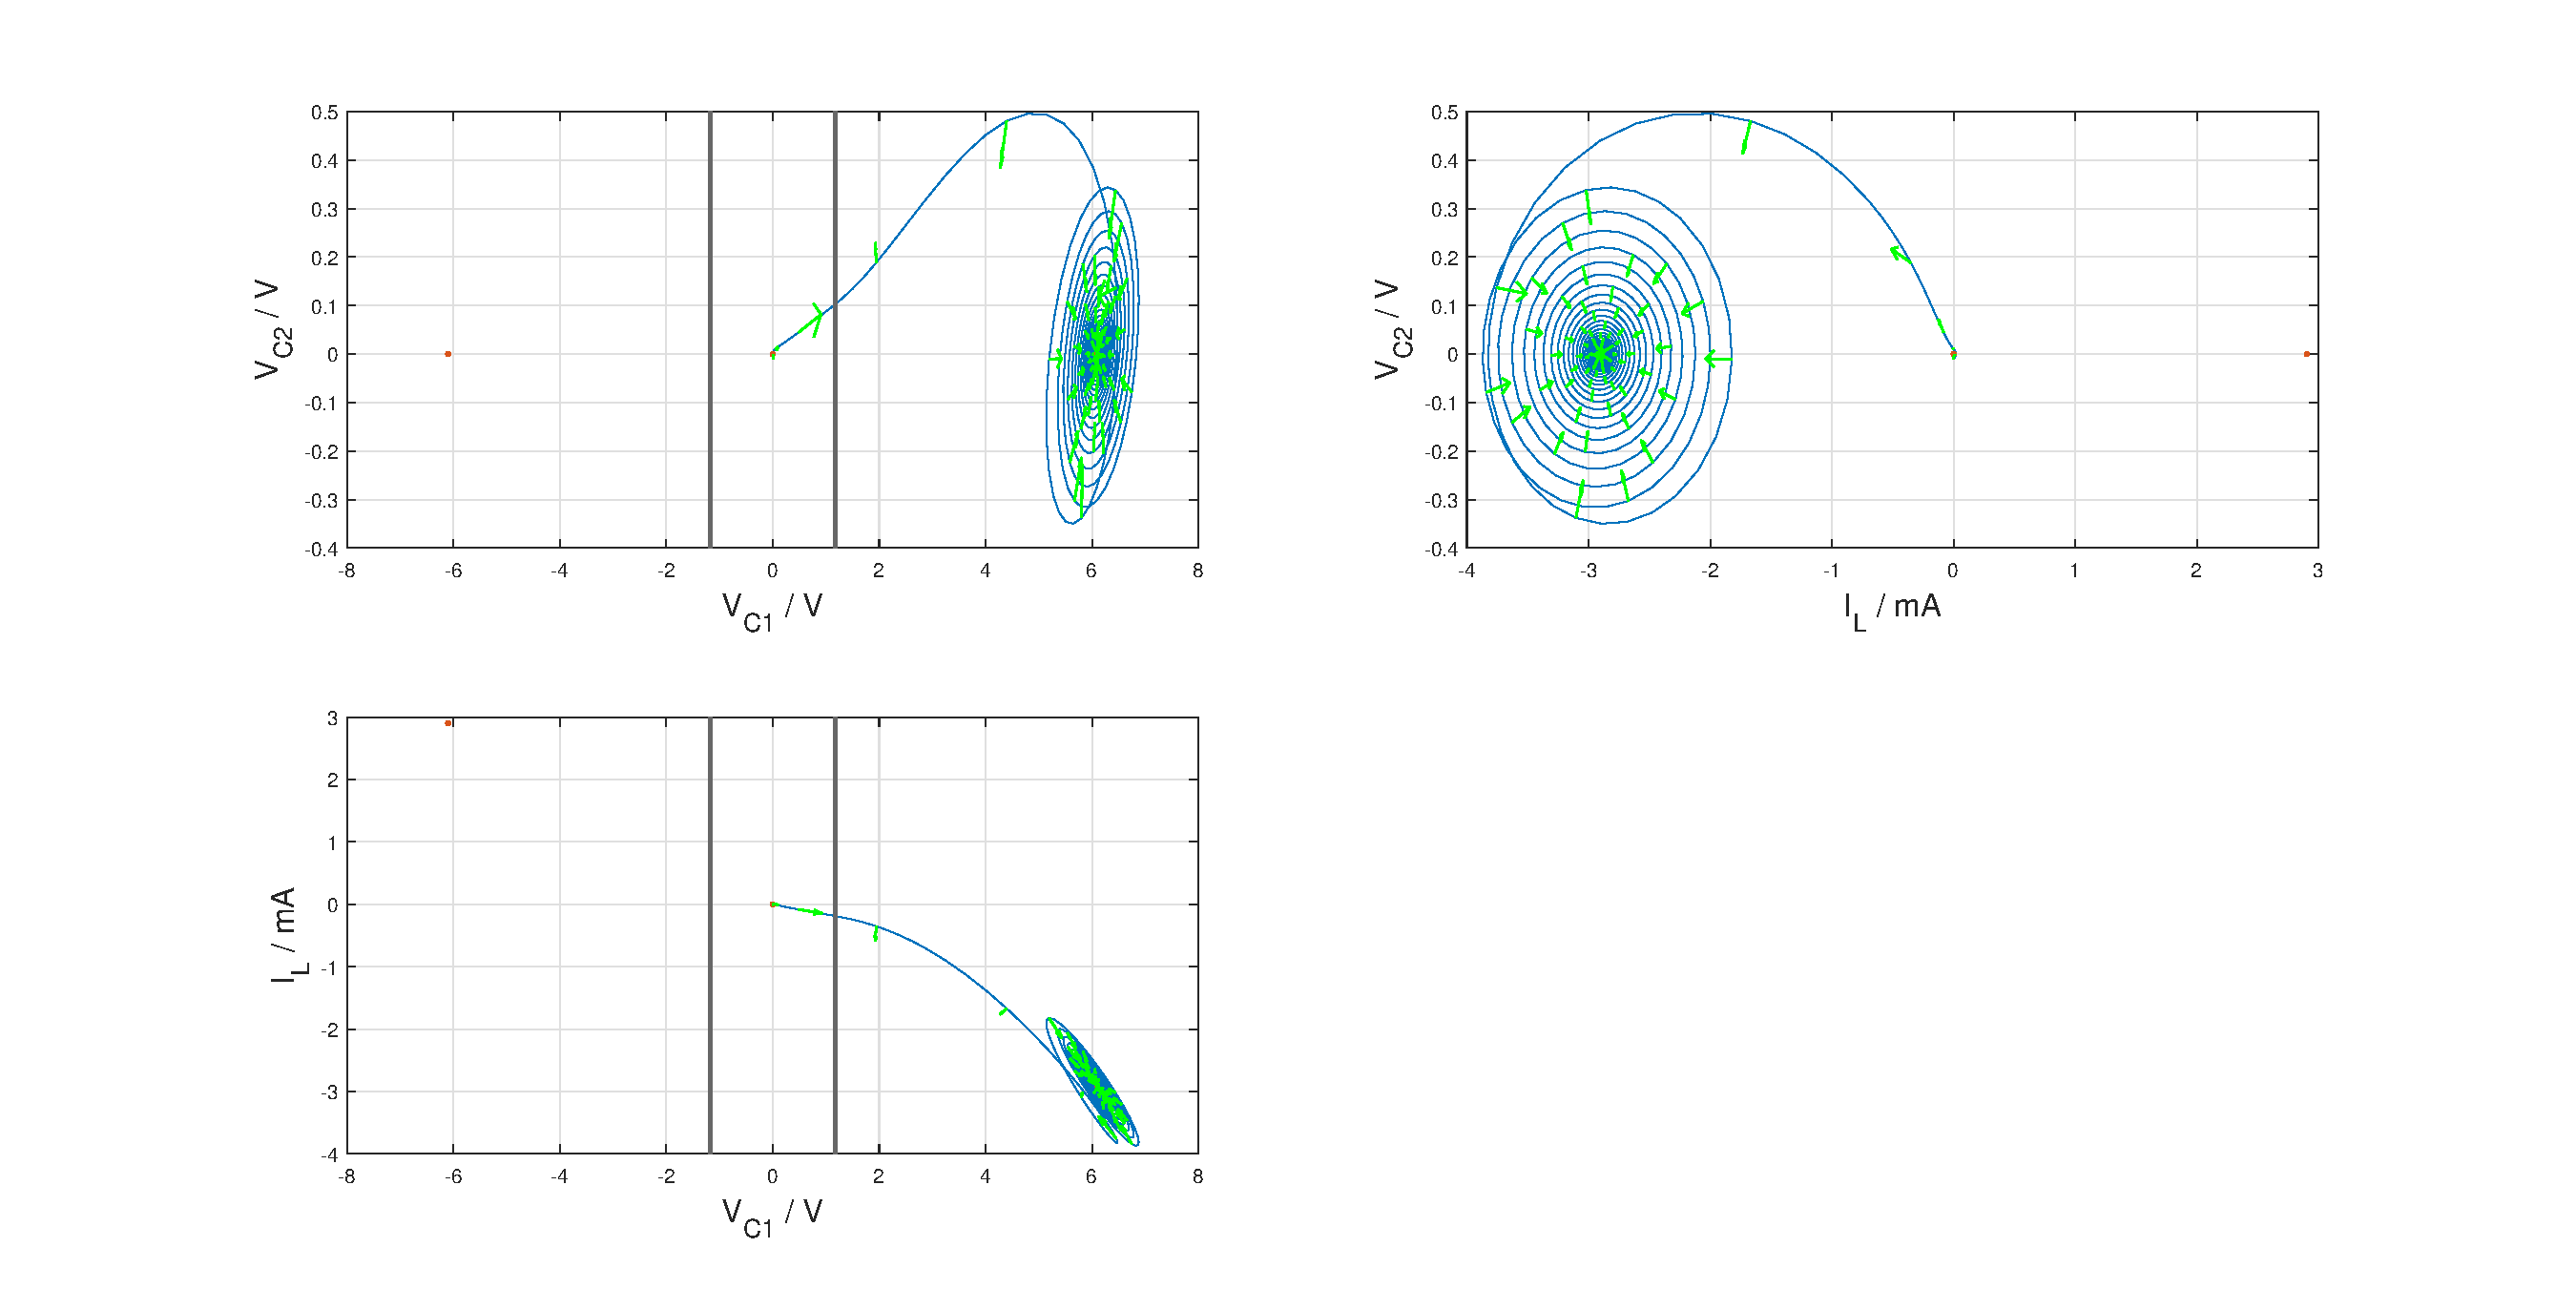
\includegraphics[width=\columnwidth]{Generalized-force-R=2100.eps}
        \caption{可变电阻阻值$R=2100\,\Omega$时,相点演化轨迹(蓝色实线)的三视图、平衡点(红点)及相点在轨迹各处受到的广义力在对应平面上的投影(绿色箭头).}
        \label{Generalized-force-R=2100}
    \end{figure}
\end{itemize}

\section{实验验证}
通过实验,我们进一步验证蔡氏电路的混动现象和以上对于蔡氏电路演化机制的解释. 我们按照图\ref{ChuaCircuit}(a)(b)(c)搭建了如图\ref{ChuaCircuit-real}所示的蔡氏电路.

\begin{figure}[H]
    \centering
    \includegraphics[width=\columnwidth]{ChuaCircuit-real.eps}
    \caption{蔡氏电路实拍,各电子元件参数已标于图中.}
    \label{ChuaCircuit-real}
\end{figure}

逐渐增大可变电阻阻值$R$,$(V_{C1},V_{C2})$点演化轨迹的变化趋势基本与第2.1小节中模拟结果一致:在可变电阻阻值$R$较小时,$(V_{C1},V_{C2})$点演化轨迹为圆角平行四边形,且随着可变电阻阻值$R$的增大,平行四边形尺寸增大,形状变得圆滑,增大电阻,如图\ref{LissajousFigure}(a)(b)(c);可变电阻阻值$R$较大时,平衡点对相点的吸引能力较强,出现双吸引子,且随着可变电阻阻值$R$增大,吸引能力增强,双吸引子的尺寸减小,如图\ref{LissajousFigure}(d)(e)(f);进一步增大可变电阻阻值$R$,平衡点对相点的吸引能力足够强从而使得$(V_{C1},V_{C2})$点演化轨迹变为单吸引子状,且随着可变电阻阻值$R$的增大,单吸引子呈现出各种不同的周期数,包括单周期、双周期、四周期和多周期.

\begin{figure}[H]
    \centering
    \subfigure[$R=110.5\,\Omega$]{
        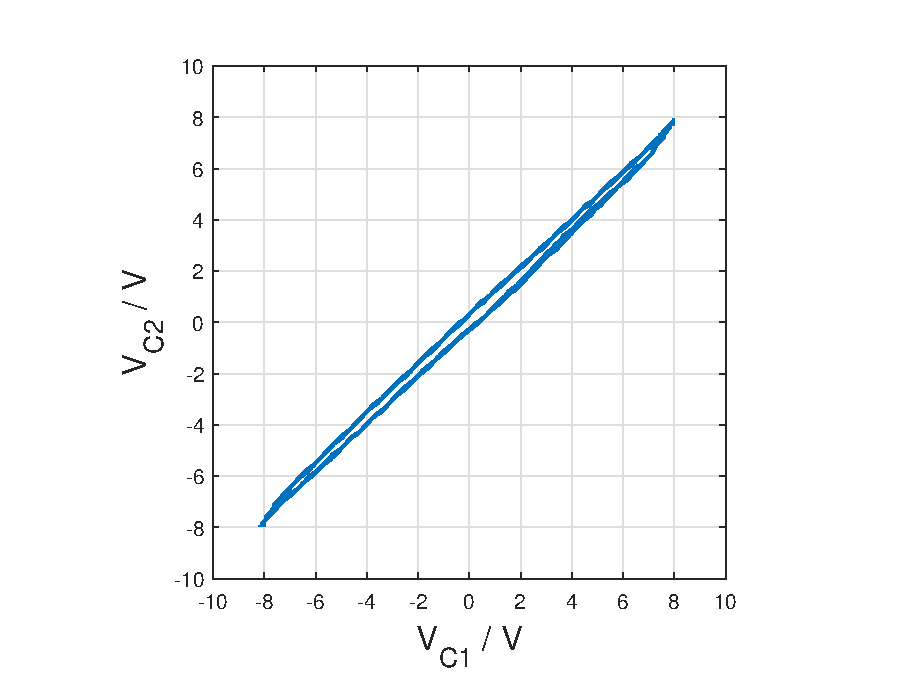
\includegraphics[width=.28\columnwidth]{R=110.5.eps}
    }
    \subfigure[$R=110.5\,\Omega$]{
        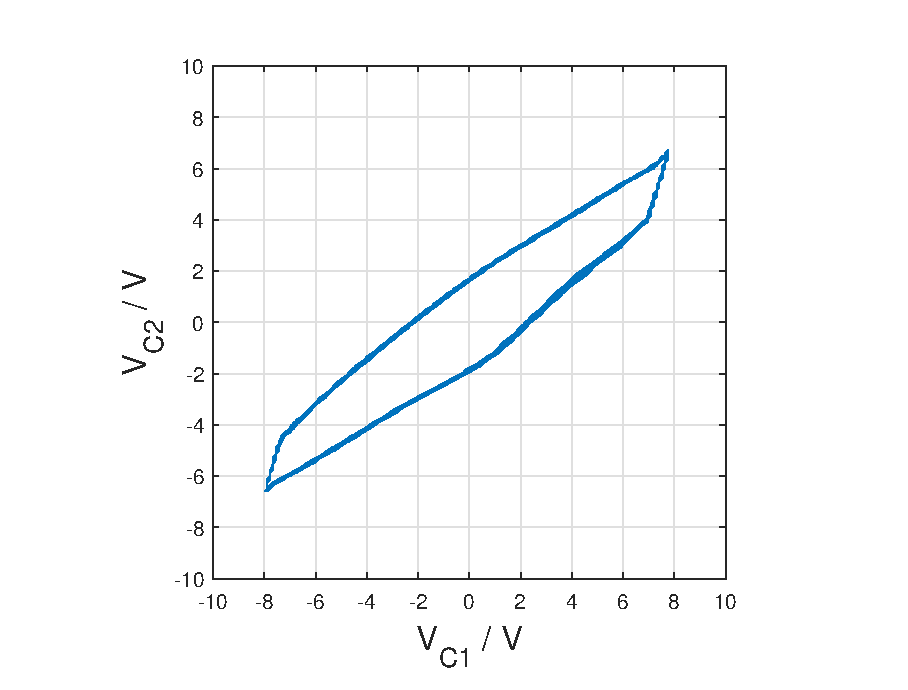
\includegraphics[width=.28\columnwidth]{R=639.eps}
    }
    \subfigure[$R=1239\,\Omega$]{
        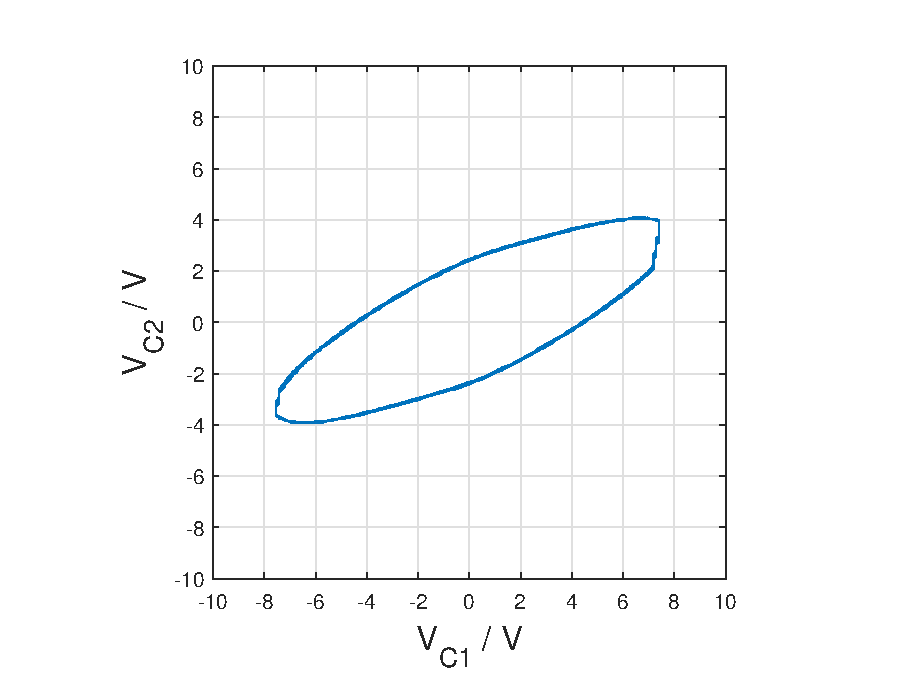
\includegraphics[width=.28\columnwidth]{R=1239.eps}
    }
    \subfigure[$R=1341\,\Omega$]{
        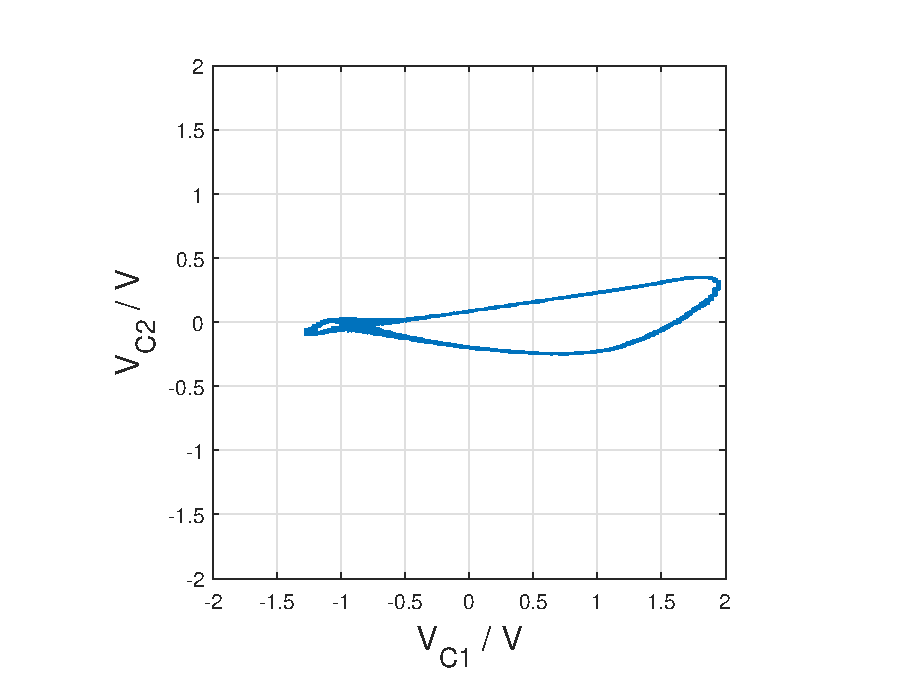
\includegraphics[width=.28\columnwidth]{R=1341.eps}
    }
    \subfigure[$R=1352\,\Omega$]{
        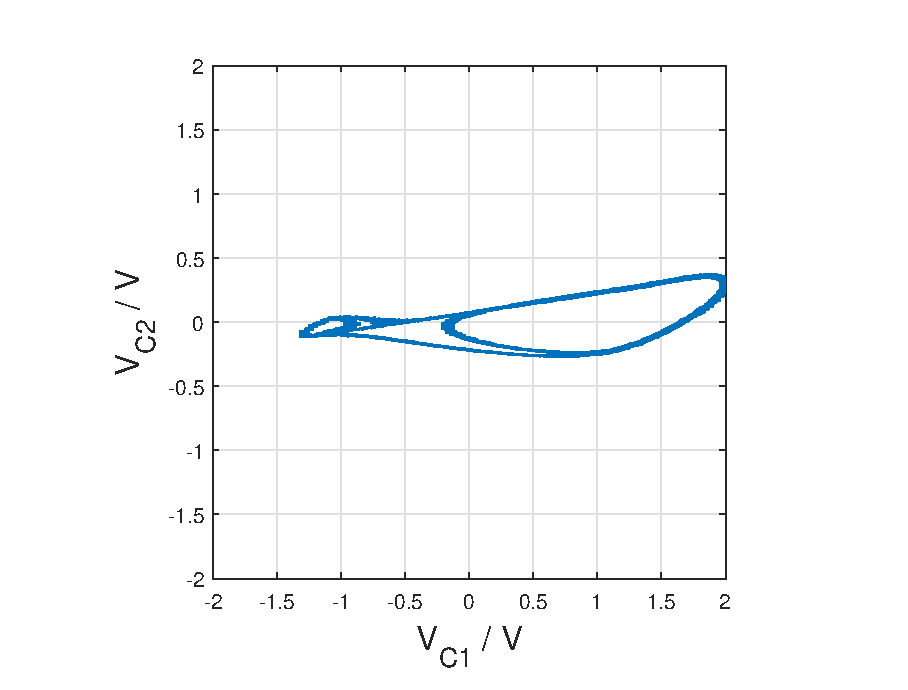
\includegraphics[width=.28\columnwidth]{R=1352.eps}
    }
    \subfigure[$R=1363\,\Omega$]{
        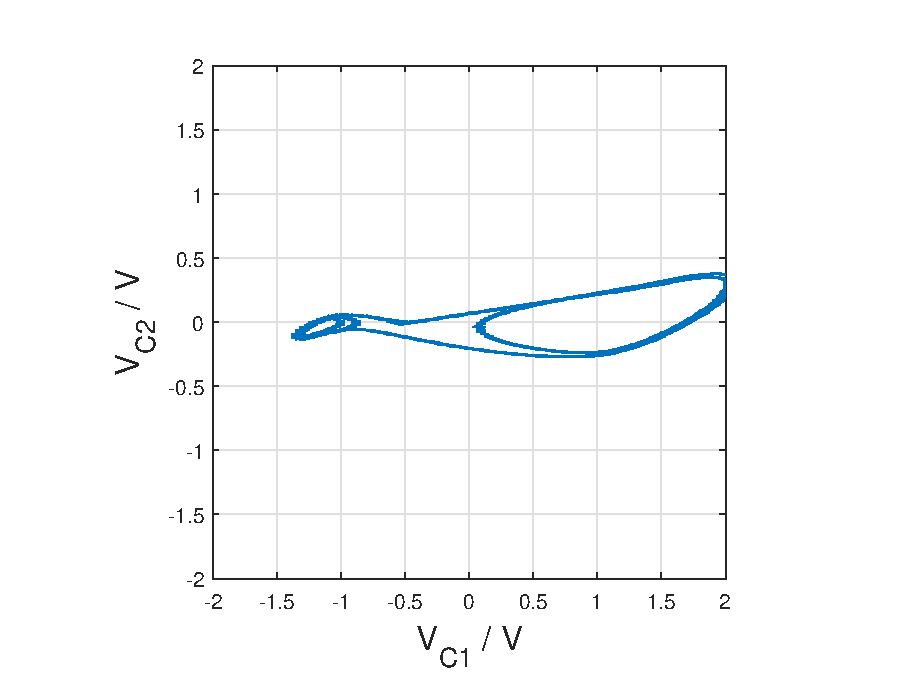
\includegraphics[width=.28\columnwidth]{R=1363.eps}
    }
    \subfigure[$R=1394\,\Omega$]{
        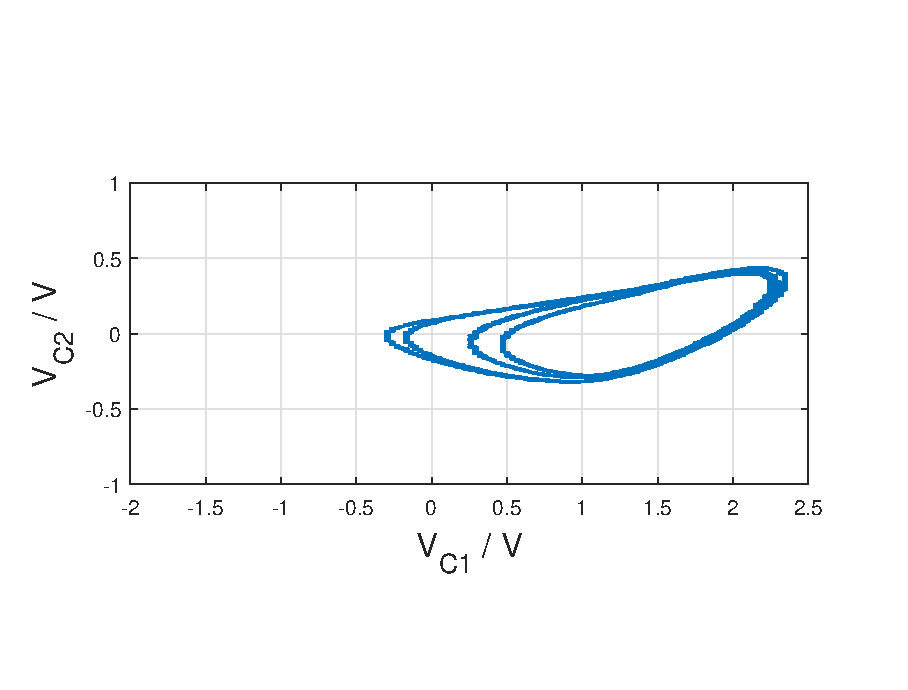
\includegraphics[width=.28\columnwidth]{R=1394-1.eps}
    }
    \subfigure[$R=1401\,\Omega$]{
        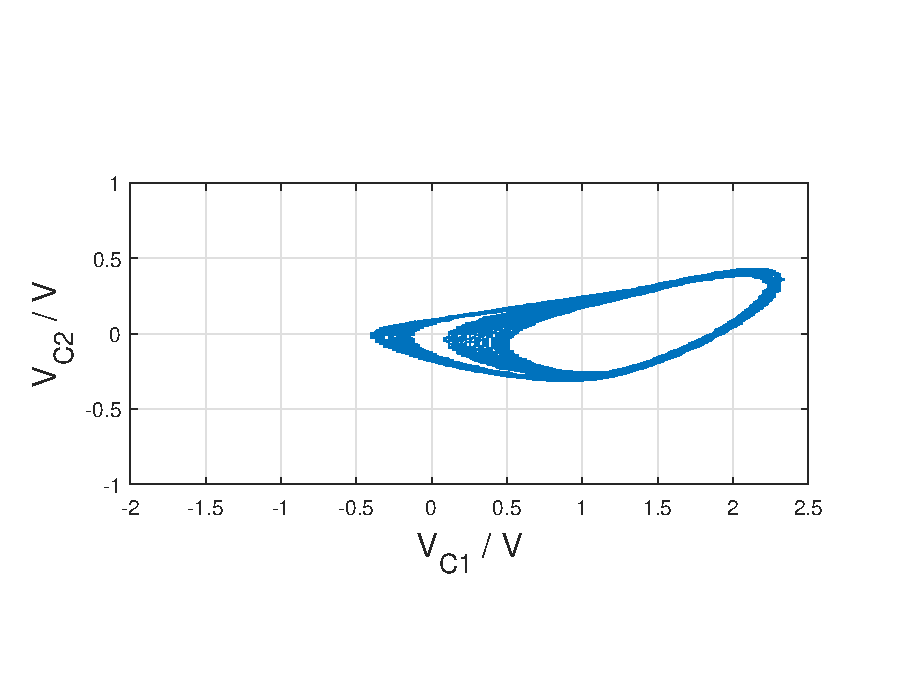
\includegraphics[width=.28\columnwidth]{R=1401.eps}
    }
    \subfigure[$R=1410\,\Omega$]{
        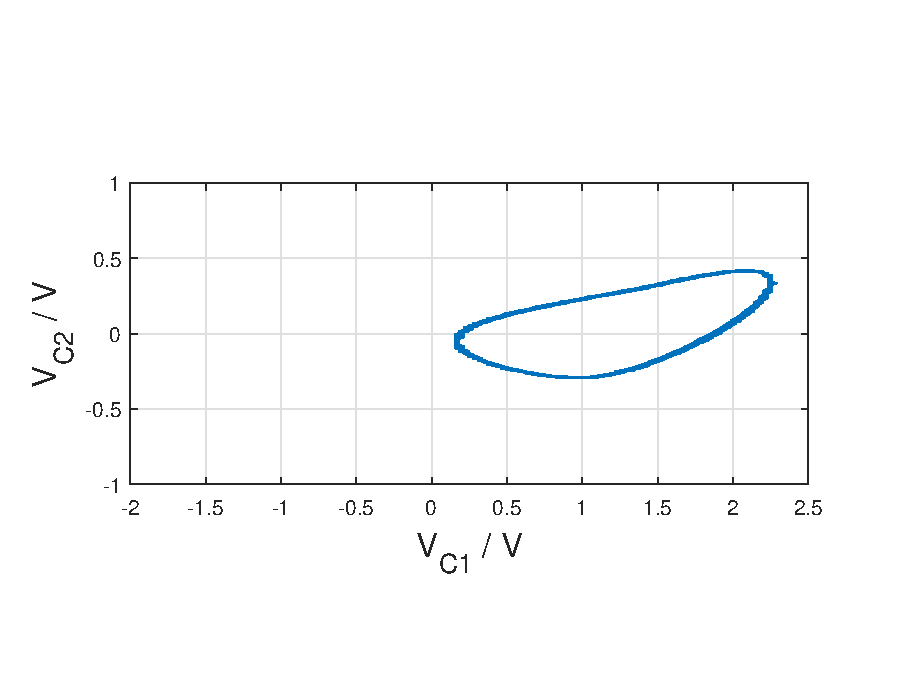
\includegraphics[width=.28\columnwidth]{R=1410-1.eps}
    }
    \caption{不同可变电阻阻值$R$的情况下,实验测得的$(V_{C1},V_{C2})$点演化轨迹.}
    \label{LissajousFigure}
\end{figure}



\end{multicols*}

\clearpage

\begin{appendix}
\section{部分未展示图片}
\begin{figure}[H]
    \centering
    \includegraphics[width=.9\columnwidth]{Generalized-force-map-R=1500-modified.eps}
    \caption{可变电阻阻值$R=1500\,\Omega$时,相空间中广义力场在不同$I_L$高度上的切片,其中绿色箭头代表广义力场在$V_{C1}-V_{C2}$平面上的投影,背景色代表广义力场沿$I_L$轴的分量.}
    \label{Generalized-force-map-R=1500}
\end{figure}

\begin{figure}[H]
    \centering
    \includegraphics[width=\columnwidth]{Generalized-force-map-R=1800-modified.eps}
    \caption{可变电阻阻值$R=1800\,\Omega$时,相空间中广义力场在不同$I_L$高度上的切片,其中绿色箭头代表广义力场在$V_{C1}-V_{C2}$平面上的投影,背景色代表广义力场沿$I_L$轴的分量.}
    \label{Generalized-force-map-R=1800}
\end{figure}

\begin{figure}[H]
    \centering
    \includegraphics[width=\columnwidth]{Generalized-force-map-R=1950-modified.eps}
    \caption{可变电阻阻值$R=1500\,\Omega$时,相空间中广义力场在不同$I_L$高度上的切片,其中绿色箭头代表广义力场在$V_{C1}-V_{C2}$平面上的投影,背景色代表广义力场沿$I_L$轴的分量.}
    \label{Generalized-force-map-R=1950}
\end{figure}

\begin{figure}[H]
    \centering
    \includegraphics[width=\columnwidth]{Generalized-force-map-R=2100-modified.eps}
    \caption{可变电阻阻值$R=2100\,\Omega$时,相空间中广义力场在不同$I_L$高度上的切片,其中绿色箭头代表广义力场在$V_{C1}-V_{C2}$平面上的投影,背景色代表广义力场沿$I_L$轴的分量.}
    \label{Generalized-force-map-R=2100}
\end{figure}

\section{Reference}
\nocite{*}
\bibliographystyle{plain}
\bibliography{References}
\end{appendix}
\end{document}